
\begin{figure}
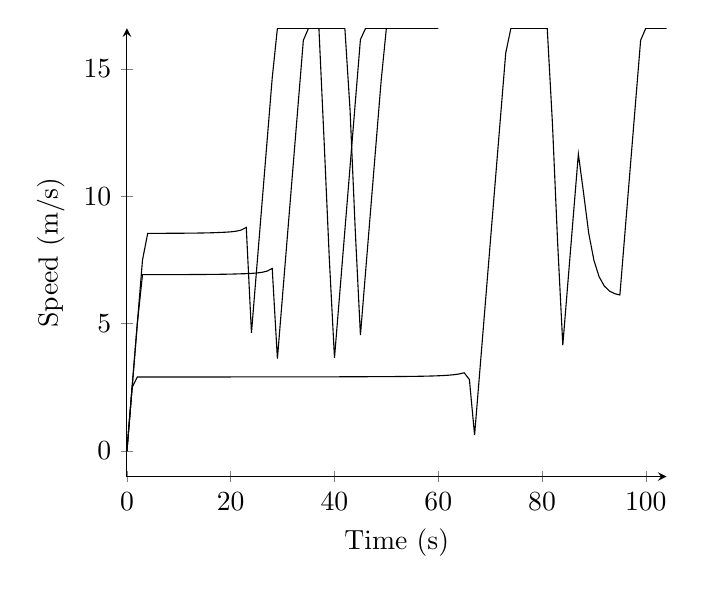
\begin{tikzpicture}
\begin{axis}[
legend style={
	anchor=west
},
axis x line=bottom,
axis y line=left,
ymin=-1,
point meta=explicit symbolic,
xlabel=Time (s),
ylabel=Speed (m/s)
]
\addplot[] coordinates {
(0, 0.0)
(1, 2.5)
(2, 5.0)
(3, 6.92495139367)
(4, 6.92526513159)
(5, 6.92561523072)
(6, 6.92600753934)
(7, 6.92644913158)
(8, 6.92694862954)
(9, 6.9275166287)
(10, 6.92816626647)
(11, 6.92891399156)
(12, 6.92978061998)
(13, 6.93079280639)
(14, 6.93198512908)
(15, 6.93340310013)
(16, 6.93510760258)
(17, 6.9371815858)
(18, 6.93974043913)
(19, 6.94294855762)
(20, 6.94704673504)
(21, 6.95239934468)
(22, 6.95957962723)
(23, 6.96446665332)
(24, 6.97482805795)
(25, 6.99062841318)
(26, 7.01657024811)
(27, 7.06404293786)
(28, 7.16798918269)
(29, 3.62601164517)
(30, 6.12601164517)
(31, 8.62601164517)
(32, 11.1260116452)
(33, 13.6260116452)
(34, 16.1260116452)
(35, 16.6)
(36, 16.6)
(37, 16.6)
(38, 16.6)
(39, 16.6)
(40, 16.6)
(41, 16.6)
(42, 16.6)
(43, 13.3976096914)
(44, 8.67978015652)
(45, 4.55170998301)
(46, 7.05170998301)
(47, 9.55170998301)
(48, 12.051709983)
(49, 14.551709983)
(50, 16.6)
(51, 16.6)
(52, 16.6)
(53, 16.6)
(54, 16.6)
(55, 16.6)
(56, 16.6)
(57, 16.6)
(58, 16.6)
(59, 16.6)
(60, 16.6)
};
\addplot[] coordinates {
(0, 0.0)
(1, 2.5)
(2, 5.0)
(3, 7.5)
(4, 8.54671079314)
(5, 8.54725879494)
(6, 8.54789070836)
(7, 8.54862459869)
(8, 8.54948367323)
(9, 8.55049814532)
(10, 8.55170793815)
(11, 8.55316669116)
(12, 8.55494784029)
(13, 8.5571540989)
(14, 8.55993270637)
(15, 8.5635008459)
(16, 8.56818982241)
(17, 8.57452575175)
(18, 8.58338604031)
(19, 8.59202811778)
(20, 8.60617969826)
(21, 8.6302655438)
(22, 8.67540342585)
(23, 8.77763663678)
(24, 4.64415790672)
(25, 7.14415790672)
(26, 9.64415790672)
(27, 12.1441579067)
(28, 14.6441579067)
(29, 16.6)
(30, 16.6)
(31, 16.6)
(32, 16.6)
(33, 16.6)
(34, 16.6)
(35, 16.6)
(36, 16.6)
(37, 16.6)
(38, 12.1694420151)
(39, 7.56817301477)
(40, 3.65801443266)
(41, 6.15801443266)
(42, 8.65801443266)
(43, 11.1580144327)
(44, 13.6580144327)
(45, 16.1580144327)
(46, 16.6)
(47, 16.6)
(48, 16.6)
(49, 16.6)
(50, 16.6)
(51, 16.6)
(52, 16.6)
(53, 16.6)
(54, 16.6)
(55, 16.6)
};
\addplot[] coordinates {
(0, 0.0)
(1, 2.5)
(2, 2.90866894617)
(3, 2.90871814255)
(4, 2.90876954085)
(5, 2.90882327454)
(6, 2.90887948736)
(7, 2.90893833428)
(8, 2.90899998259)
(9, 2.90906461307)
(10, 2.90913242134)
(11, 2.90920361934)
(12, 2.90927843698)
(13, 2.90935712402)
(14, 2.90943995216)
(15, 2.90952721739)
(16, 2.90961924263)
(17, 2.90971638077)
(18, 2.90981901803)
(19, 2.90992757785)
(20, 2.91004252525)
(21, 2.91016437186)
(22, 2.91029368162)
(23, 2.91043107736)
(24, 2.91057724834)
(25, 2.91073295896)
(26, 2.91089905878)
(27, 2.91107649423)
(28, 2.91126632215)
(29, 2.91146972568)
(30, 2.91168803281)
(31, 2.91192273823)
(32, 2.91217552916)
(33, 2.9124483159)
(34, 2.91274326833)
(35, 2.91306285943)
(36, 2.91340991767)
(37, 2.91378769033)
(38, 2.91419992036)
(39, 2.91465094022)
(40, 2.91514578727)
(41, 2.91569034648)
(42, 2.91629152802)
(43, 2.91695749013)
(44, 2.91769792078)
(45, 2.91852439672)
(46, 2.91945084529)
(47, 2.92049414428)
(48, 2.92167490923)
(49, 2.92301853883)
(50, 2.92371741227)
(51, 2.92446477368)
(52, 2.92594649641)
(53, 2.9276799189)
(54, 2.92972604109)
(55, 2.93216575147)
(56, 2.93510825856)
(57, 2.93870407678)
(58, 2.94316566597)
(59, 2.9488014683)
(60, 2.95607456353)
(61, 2.96570930677)
(62, 2.97889859632)
(63, 2.99774301386)
(64, 3.02629614139)
(65, 3.07350781666)
(66, 2.80755503127)
(67, 0.624376593581)
(68, 3.12437659358)
(69, 5.62437659358)
(70, 8.12437659358)
(71, 10.6243765936)
(72, 13.1243765936)
(73, 15.6243765936)
(74, 16.6)
(75, 16.6)
(76, 16.6)
(77, 16.6)
(78, 16.6)
(79, 16.6)
(80, 16.6)
(81, 16.6)
(82, 12.871002395)
(83, 8.20079936667)
(84, 4.16135376082)
(85, 6.66135376082)
(86, 9.16135376082)
(87, 11.6613537608)
(88, 10.135779362)
(89, 8.54622555161)
(90, 7.4870346021)
(91, 6.84218602648)
(92, 6.47742020467)
(93, 6.28139055338)
(94, 6.17937901181)
(95, 6.12735989419)
(96, 8.62735989419)
(97, 11.1273598942)
(98, 13.6273598942)
(99, 16.1273598942)
(100, 16.6)
(101, 16.6)
(102, 16.6)
(103, 16.6)
(104, 16.6)
};

\end{axis}
\end{tikzpicture}
\label{tik:50:21_V, 20_V, 17_N, 15_S, 15_S.-30, 15_N, 16_V}
\caption{50 percent diving with GSC on route $21_V, 20_V, 17_N, 15_S, 15_S.-30, 15_N, 16_V$}
\end{figure}
